%BCOR: BindeKorrektur. Sie macht den Rand auf der Seite an der das
%      Werk gebunden wird gr��er.
%DIV:  ist bei einer 11pt schrift standardm��ig auf 10 eingestellt, und
%      ist ein Ma� f�r den beschreibbaren bereich. Je gr��er der Wert,
%      desto gr��er der schreibbare Bereich und desto kleiner die
%      R�nder
\documentclass[a4paper,twoside,12pt,DIV10,BCOR=15mm,appendixprefix,final,
							 accentcolor=tud5b,colorback,longdoc,bigchapter,firstlineindent]{tudreport}

%Deutsche Rechtschreibung und Schriftarteinstellungen
%\usepackage[ngerman]{babel}
\usepackage[latin1]{inputenc}
\usepackage[T1]{fontenc}
\usepackage{textcomp}

% Grafiken, Tabellen, lange Tabellen
\usepackage[]{graphicx,color}
\usepackage[]{array}
\usepackage[]{tabularx}
\usepackage[]{longtable}
\usepackage[]{booktabs}

%Neudefinition des Abstandes zwischen 2 cmidrules, d.h.
%den mittleren Trennstrichen innerhalb von Tabellen
\cmidrulesep=0.5\doublerulesep
\usepackage[]{subfigure}
%\usepackage[]{epsfig}
\usepackage[]{rotating}
%Ams-tex Paket f�r erweiterte Mathematik-Umgebungen
\usepackage[]{amsmath}
%\usepackage[]{amssymb,amsfonts,amsxtra}
\usepackage[]{theorem}

%Darstellung von Code
\usepackage[]{verbatim}
\usepackage[]{moreverb}
\usepackage[]{latexsym}

%Darstellung von Algorithmen
\usepackage[ruled,chapter]{algorithm}
\usepackage[]{algorithmic}

%Setzen der Alg.Benennungen von engl.-->dt.
\floatname{algorithm}{Algorithmus}
\renewcommand{\listalgorithmname}{Liste der Algorithmen}

%Literaturverzeichnis (Stil der Referencen)
%\usepackage[square,sort&compress]{natbib}

\usepackage{tikz}
\usepackage{pgfplots}

% Pfad entlang dem die Bilder gesucht werden.
\graphicspath{{images/}}

% Label einer Abbildungs- oder Tabellenunterschrift fett
\addtokomafont{captionlabel}{\bfseries\sffamily\small}

% Einheiten fuer Bilder (picture-Umgebung)
\unitlength1mm

% Die Folgenden Einstellungen sollten an die vorliegenden Bedingungen
% angepasst werden:

% Tiefe der Gliederung
%\setcounter{secnumdepth}{5}

% Tiefe des Inhaltsverzeichnisses
%\setcounter{tocdepth}{4}

% --- Trennmuster fuer Ausnahmefaelle
%\hyphenation{Lern-al-go-rith-men}
%\hyphenation{Schur-Kom-ple-ment}
%\hyphenation{Volumen-Pen-al-ty-For-mulier-ung}
%\hyphenation{elasto-plas-tische}

% Definition von Theorem-Umgebungen
\theoremstyle{break}
\newtheorem{definition}{Definition}[section]
\newtheorem{theorem}{Theorem}[section]
\newtheorem{satz}{Satz}[section]
\newtheorem{beweis}{Beweis}[section]
\newtheorem{schluss}{Schlu"sfolgerung}[section]
\newtheorem{beispiel}{Beispiel}[section]


\title{%
  Combining Rigid body simulations with oriented particles
}

\subtitle{%
  Bachelor's thesis
}

\institution{%
TU Darmstadt
}

% enter file name without extension eps/pdf
\setinstitutionlogo[height]{%
gsclogofull%
}

%\dedication{%
%To my incredibly patient wife.
%}

%\uppertitleback{%
%
%}

\lowertitleback{%
Technische Universit�t Darmstadt, 2012
}

%\settitlepicture{%
%GSCKeyVisualreport.eps
%}


%%%%%%%%%%%%%%%%%%%%%% HAUPTDATEI %%%%%%%%%%%%%%%%%%%%%%%%%%%%%%%%%%%%%%%%%%%%
\begin{document}

%**** Titelseite und eidesstattliche Erkl�rung****
\pagestyle{empty}
\maketitle{}
\cleardoublepage
\vspace*{130mm}
%\hspace*{70mm}
\begin{minipage}{129.5mm}

  I declare that I have authored this thesis independently under the
  supervision of Prof.~Dr.~Jan~Bender and Crispin~Deul,~M.Sc.
  and that I have only used the quoted or referenced resources. \\ [20mm]

Darmstadt, den \today

\end{minipage}
\renewcommand{\thepage}{\arabic{page}}
\setcounter{page}{1}
\newpage

%%% Local Variables: 
%%% mode: latex
%%% TeX-master: "main"
%%% End: 



\cleardoublepage
%******  Abstract **************
\begin{abstract}
The major objective of this study is to explore the possibility of combining a traditional rigid body simulation with a deformable body simulation. The deformable bodies are implemented according to the relatively new approach of using oriented particles. The combined bodies consist of a rigid inner structure and a soft outer structure. The goal is to improve upon traditional system simulating skeletons. The bones can now be modeled with a surrounding cushion of tissue using the presented method. This extends and improves simpler models using only rigid bodies especially in areas where the number of contact points is important to achieve a stable simulation.  Using the soft deformable tissue enables bodies to surround other bodies more realistically while increasing the number of contact points significantly. Thus this combined simulation model thus can provide a more stable simulation.

The main contribution of this thesis is the modeling and description of the interface between the deformable oriented particles and rigid bodies. The first interface is inside the body itself, between the bones and the tissue which requires an efficient way to closely couple both subsimulations. The second interface is between these combined bodies and rigid bodies in the simulated world. Here the impulses generated by the tissue onto the rigid bodies has to be defined and calculated.

The outcome shows that the simulation provides realistic results. For the simple scenario of picking up a cylinder only two rigid bodies, modeling the fingers, are needed. A rigid body only simulation would either completely fail at this task or would require multiple bodies to simulate the whole finger. This result promises both more efficient and faster simulations of complete skeleton models.
\end{abstract}

\cleardoublepage

% ***** Wichtige Seiten *****
\pagenumbering{roman}
\tableofcontents
\listoffigures
%\listoftables

% sofern vorhanden, einkommentieren:
\listofalgorithms
%\include{symbolverzeichnis}
\newcounter{roman_counter}
\setcounter{roman_counter}{\value{page}}

%*****Beginn der eigentlichen Arbeit********
\clearpage

%\pagestyle{scrheadings}
\setcounter{page}{1}
\pagenumbering{arabic}

\chapter{Introduction}
\label{cha:introduction}

Simulating physically properties of objects with the help of a computer is a very important topic across a wide range of fields. As computing power is both expensive and limited, the approach to simulations is distributed across a spectrum of accuracy at the one end and performance on the other. Some fields require the best and most accurate simulations currently available. These are especially predominant in applications where predictions of the real world behavior of the system are required and later applied to constructing and optimizing real world objects. Example fields for this are automotive or aerospace modeling and simulations. Here extremely detailed models are used to predict the properties and behaviors of all kinds of different materials, shapes and bodies. The results of these simulations directly influence the construction and design decisions for their real world counter parts. Simulating the objects inside the computer first enables a faster development cycle and thus provides an efficient and cost effective way of constructing new parts and pieces.

Other fields are not as reliant on the direct applicability of their results to the real world. The main focus of these simulations is to provide physically plausible and visually believably results in a timely fashion. Probably the two most popular and widely known application for these types of simulations are games and animations. Here the goal is to introduce the viewer to a completely virtual universe where the media creators control everything. In order to achieve the desired immersion of the viewers realistic behavior the actors and objects is really important in this universe. Obvious incorrect physical behavior is most of the time immediately recognizable by the consumers and can easily break their immersion in the content.

Nowadays games and animations use a large number of interacting bodies. These bodies are simulated using a variety of different simulation methods and techniques. For animating characters and objects in movies the main focus lies in reducing the workload of animators, who traditionally had to animate and model everything by hand, a long and tedious process. Physical simulations can aid the animators by automatically generating physically plausible animations to start off with. These animations can then later be adjusted and modified as necessary but the simulation can do a huge amount of work. These techniques and methods are only secondarily focused on the simulation time. While this is still a consideration to enable faster turn around times for the animator playing with different ideas the primary focus of these systems is the controllability of the output. These system should enable the animators to define their desired behavior and let the system automatically figure out how to simulate everything in between, always trying to have an at least physically plausible result.

Physical simulations in games however have to primarily focus on the real time aspect of their respective techniques and methods. Today's games simulate a large a amount of objects in an ever-increasing world. All these simulations have to be calculated in an extremely short period of time. The simulated physics have to share the resources with everything else required to simulate the game world including game logic, artificial intelligence and computer graphics. In order to achieve smooth 60 fps all these different subsystems have to be extremely efficient and fast. If the simulations slow down too much the immersion of the player will be broken immediately broken when things start to move unrealistically.

Another interesting subarea of the games are the so called serious games. Here the focus of the simulated world lies not on providing fun and entertainment to the player. Instead the goal is to model the real world as realistically as possible to enable training and orientation for people working in the simulated field of expertise. Prominent examples are military and emergency personnel. Simulations can be used to give these people the opportunity to experience real world scenarios in a controlled environment so they can train and prepare for their duties. These kinds of games are also used to help train medical personnel to perform surgeries on completely simulated patients first before applying the knowledge to real world cases. Providing realistic real time feedback to the users is the main focus of these types of simulations.

For all close to real time and controllable simulations rigid body simulations have been a very popular choice. Rigid body simulations enable fast and efficient simulations of a huge number of interacting bodies. This can be achieved with the assumption that all bodies in the simulation are completely rigid and can never deform. This assumption is plausible for a wide variety of applications ranging from simple car models to more complex ragdoll models. Unfortunately not all possible scenarios can be modeled with simplified rigid bodies. Objects in the real world are very often deformable and bend and stretch under the influence of external forces. Incorporating deformable simulations models into games and animations enable a whole new range of interesting scenarios. However the simulation of deformable bodies requires a lot more computing resources to achieve realistic results. Novel ways to reduce the amount of work associated with deformable simulations have to be found.

One such approach is to combine the two different simulation approaches. Here the goal is to combine the very fast rigid body simulations with the slower deformable simulations in order to reap the benefits of both simultaneously. Some approaches try to simulate rigid bodies and deformable bodies side by side for each object, while other approaches try to model a single body using both rigid as well as deformable parts. A real world example of the second one is the human body itself. Here basically rigid bodies, the bones, form an underlying rigid skeleton. However in contrast to simple ragdolls, in reality a soft layer of tissue surrounds this rigid skeleton. This soft tissue can deform when forces are applied. Modeling this seemingly obvious scenario efficiently is non trivial and a perfect match for a combined simulation model.

The focus of this thesis is to explore this type of simulation, where a rigid inner core is simulated with a soft outer layer of deformable material. The goal is to achieve an efficient simulation, which is both fast and robust in scenarios where using only a simplified rigid body simulation would offer unsatisfactory results. The thesis furthermore focuses on a specific technique to implement the deformable material. This technique uses oriented particles to simulate the deformations of a body. Oriented particles can be simulated efficiently and in real-time while still giving physically plausible results.

The thesis first gives a short background on how rigid body simulations are implemented and how the simulation is used in the proposed method. Following, a more in-depth description of the way oriented particles are implemented is presented, beginning with position based dynamics and shape matching and explaining how these approaches enable oriented particles. The next part describes the method and ideas for combining these two different approaches into one system. Finally, a demo application is implemented and different scenario using the proposed method are illustrated.
\chapter{Problem Analysis}
\label{cha:problem_analysis}

This thesis focusses on a concrete example scenario. This helps to better understand the implications and advantages of the proposed method. Also the obtained results are more easily compared against the traditional approach.

A widely applicable scenario for modeling bones and soft tissue are fingers. The scenario being used in this thesis involves two fingers grabbing onto and lifting block of the ground. The fingers are positioned to the either side of the block in the model. While applying a continuous pressure onto the block the fingers are lifting it up from the floor and into the air. This is directly applicable to a number of different scenarios involving a robotic arm with attached fingers, which is supposed to pick up blocks are other objects of the ground.

image

illustration of scenario

image


All this has to be able to be simulated in realtime in order to be used games and animations. The simulations also has to be robust against numerically instabilities. These are either caused by simple numerical or rounding errors or by the fingers being slightly off the target when grabbing onto the block. Forces between the inner bone and outer tissue as well as forces between the tissue and other objects have to be modeled so a realistic result can be achieved. This is especially true for the friction caused by the tissue on the block, as otherwise the block would not be lift up at all.

Using a simple rigid body simulation for this is suboptimal. Both fingers and the block would be modeled as rigid bodies. Resolving all the resulting forces acting on the block can quickly get numerically unstable. The blocks can start to move and wiggle incorrectly until the results are no longer visually pleasing and physically plausible.

The problem is further complicated when instead of a simple block any kind of round object like a cylinder would have to be picked up. This would require the fingers to be touch the cylinder perfectly perpendicular and on the exact opposite points. Otherwise the pressure and the resulting forces would simply let the cylinder slip out either in front or the back. This is basically impossible to achieve numerically.

The way to traditionally solve this problem has been to use multiple rigid bodies to simulate the each finger to get a better grip on the object that is lifted up. This way complicates the simulations quite a bit as joints and and many more blocks have to be simulated. However the problem of slowing increasing numerically instabilities would still occur and might still be very hard to handle efficiently.

Solving the problem with only deformable bodies is theoretically possible, however this would not really capture the real world idea of a rigid bone structure with a surrounding soft layer of tissue. Simulating everything as a deformable body would not be very efficient. This would require a lot more computational resources, especially when considering to apply this to a complete skeleton. Great care has also be taken to ensure that some deformable parts are mostly behaving as rigid structures while still giving a physically plausible result.

Therefore the main requirements for the proposed technique of combining an inner core of rigid bodies with a soft layer of surrounding deformable material can be summarized as:

\begin{enumerate}
\item realtime simulation
\item	low number of bodies
\item only approximate orientation of the fingers relative to the block
\item collision handling/force propagation inside the body between "bone" and "tissue"
\item modeling friction between fingers and object
\end{enumerate}
\chapter{Related Approaches}
\label{cha:related_approaches}

The approach described in this thesis uses oriented particles to simulate soft tissue around a rigid inner bone. The combination of rigid body simulations with deformable body simulation were explored very early by Terzopoulos et al. \cite{Terzopoulos:1988bz} shortly after deformable bodies were first introduced in \cite{Terzopoulos:1987gf}. Since then many different techniques and methods have been researched. A recent review of different approaches can be found in \cite{Nealen:2006vp}. The work in this thesis builds upon particle based simulations and in particular the approach by M{\"u}ller et al. \cite{Muller:2011gn}. The approach itself combines and extents the two previous methods of shape matching described in \cite{Muller:2005fi} and position based dynamics found in \cite{Muller:2007vs} by additionally including the orientation of each particle into the calculations.

There are two different ways of approaching the combination of rigid body simulations and deformable body simulations. The first focusses on a two-way coupling of the bodies. This means each body is simulated using its own simulation. Both types are then allowed to interact in the same simulation world. For example Jansson et al. \cite{Jansson:2003cb} used a mass-spring representation extended by the concept of volume to simulate both rigid bodies and deformable bodies. Thus they had no need to explicitly handle the interaction as both types of bodies used the same underlying representation.

Lenoir et al. \cite{Lenoir:2004ic} explored a more generic constraint solver using Lagrange theory to simulate deformable models and a classical Newton-Euler formalism to simulate rigid bodies. In 2007 both \cite{Muller:2007vs} and \cite{Sifakis:2007to} extended their respective frameworks to handle two-way coupling between rigid and deformable bodies. Another improvement followed in \cite{Shinar:2008va} which focused on the stability of coupling. They achieved this by using a unified time integration for both simulations as well as an individual two-way coupling algorithm for each body type.

The second approach for combining rigid bodies with deformable bodies focuses on modeling an inner skeleton to drive the outer deformable parts. One of the first of such ideas was explored in \cite{Capell:2002ge}. They utilized the finite element method (FEM) to simulate the deformable body but in addition introduced line constraints along the bones of the skeleton. Later Georgii et al. picked up on this general idea in \cite{Georgii:2010tw} by including a more advanced two-way coupling algorithm based on a geometric multigrid scheme to solve the FEM equations governing the deformable body parts.

In the paper \cite{Jain:2011hb} Jain et al. explore a very similar approach to the one taken in this thesis. They also use articulated rigid bones and surround them with a set of point masses that simulate the deformable body parts. Improving the performance of these types of simulations with an inner skeleton is the main focus of \cite{Kim:2011iq}. Instead of point based deformable bodies they choose to implement non linear finite elements in order to negate the problems arising from the linearized stress when the deformations contain rotational modes. A problem which is also addressed by incorporating the orientation information into the deformable model as done by the oriented particles approach in \cite{Muller:2011gn}. 

Another interesting paper by Stavness et al. \cite{Stavness:2011fn} explores the application of skeleton based deformable models to simulate real world body parts for medical applications, including a FEM model for the tongue, muscle actuators, constraints for the bite contact and rigid bones for the jaw.

Applying rigid skeletons combined with soft deformable outer layers to the field of computer animation is the focus of a paper by McAdams et al. \cite{McAdams:2011ht}. They utilize a hexahedral lattice to simulate the deformable skin of the animated character, which is solved by using a multigrid method. M{\"u}ller et al. themselves extend upon their original oriented particles approach in \cite{Muller:2011vu}. They present a method to apply oriented particles to enhance the realism of animated characters. However, instead of explicitly modeling the bones as rigid bones, they link the particles to a regular mesh representing the underlying skeleton structure.
\chapter{Fundamentals}
\label{cha:fundamentals}

This section describes the fundamental buildings blocks of the algorithm described in this thesis. It provides a quick overview and explanations of how the two different simulation techniques work. It does not describe in any way how the two different simulations might interact but instead describes them in total isolation.

\section{Rigid Body Simulations}
\label{sec:rigid_body_simulations}

Rigid bodies simulations is very similar to simple particle simulations. Simple particles are modeled as infinitesimal point masses, rigid bodies additional are defined by their dimension. This extension in space remains constant through out the whole simulation. A rigid body can therefore be thought of like a set of many particles. If a force is acting on any one of these point masses all the other connected masses in the rigid body are affected as well. Each point mass has a fixed mass $m_i$ and is located at fixed position $r_i$ inside the system. The total mass of the rigid body is then simply the sum of all the point masses combined

\[
M = \sum\limits_{i=1}^N m_i
\]

The position of the particles is defined relative to a local body coordinate system. The origin of coordinate system is the center of mass of the rigid body. The center of mass is calculated as 

\[
c = \frac{\sum m_i r_i}{M}
\]

In order to describe a rigid body simulation two variables are of central importance. First is the position \(x(t)\) of the rigid body in space. The second is the orientation \(q(t)\)in space. Both these variables are defined in relation to the world coordinate system. There are two different approaches to model the orientation of the rigid body, either a rotation matrix $R(t)$ or a unit quaternion $q(t)$. In practice in almost all cases unit quaternions are used for a number of reasons. One important aspect is the fact that quaternions don't suffer from gimbal lock like simple Euler angles do. Another aspect is that a quaternion consists of only 4 numbers instead of the 9 numbers required for a full rotation matrix. This second point leads to both easier and more efficient calculations, especially for interpolation and normalization.

\begin{figure}[htbp]
\centering
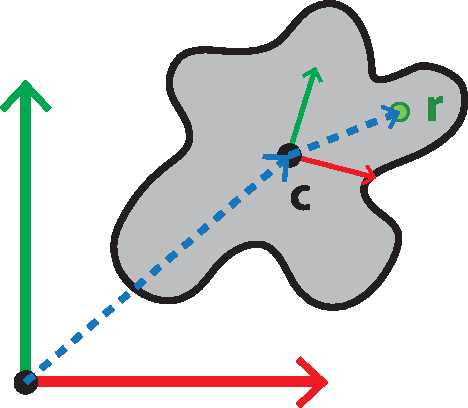
\includegraphics[width=.4\textwidth]{images/rigid_body_1.pdf}
\caption{Rigid body model illustration}
\label{img:rigid_body}
\end{figure}

By definition only the affine transformations of rotation and translation can apply to any rigid body. The main task of the rigid body simulation is therefore to calculate these to variables over time \(t\).

The physics behind the rigid body simulation is based on Newton's laws of motion. Most importantly the first law stating that if no force is acting on an object, the velocity of the object will remain constant. Thus follows that the simulation has to model all forces acting on the body. These forces are the only causes for a change in the bodies state and thus its position and orientation in space. The forces either cause a change in the linear velocity of the body, or an angular velocity results in a rotation of the body. 

The position of the rigid body is defined by the position $x(t)$ of its center of mass in world coordinates over time. The change of this position over time defines the linear velocity $v(t)$ for the body. So the linear velocity is simply the following.

\[
v(t) = \dot{x}(t)
\]

The angular velocity is a little harder to define. First the current rotation of the body has to be stated. The orientation of the rigid body was defined as unit quaternion $q(t)$. The change in orientation can than be calculated with the following .

\[
\dot{q}(t) = \omega(t) * q(t)
\]

Here $\omega(t)$ denotes the angular velocity of the body at any point in time. Both the linear velocity and the angular velocity are integrated in every time step to simulate the bodies behavior.

So in its most basic form the state of a rigid body body is defined by just the following five variables

\begin{align*}
m &, \text{the mass} \\
x &, \text{the position of the center of mass} \\
q &, \text{the orientation} \\
v &, \text{the linear velocity} \\
\omega &, \text{the angular velocity} \\
\end{align*}

Until now only the state of the rigid body has been defined. In the real world force are acting upon the body which cause a change in its state according to Newton's laws of motion. The most prominent force usually modeled in a rigid body simulations are for example gravity, collision and friction. In the real world force always act over a defined amount of time. Unfortunately for the simulation an instantaneous change in velocity is more desirable, so that for example in the case of collision the relative velocity of the involved bodies comes to a hold immediately. In order to achieve this goal the new quantity $J$ is introduced. $J$ is called an impulse and represents a force integrated over time.

\[
F \Delta t = J
\]

Letting $F$ go to infinity and $\Delta t$ to zero describes how the force would change the velocity if it would cause an immediate change. $J$ thus has the units of momentum. 

Again the effects of any impulse has to be evaluated for both the linear velocity as well as the angular velocity. For the linear velocity the change is rather defined as

\[
 v(t) = \frac{P(t)}{M}
\]

In this case $P(t)$ denotes the linear momentum aggregated across all force acting upon the body and $M$ is simply the mass of the rigid body.

The formula for the angular velocity again is a little more involved

\[
\omega(t) = L(t) * inv(I(t))
\]

Here $L(t)$ denotes the angular momentum. $I(t)$ is called the inertia tensor and is a simple scaling factor between the angular momentum $L(t)$ and $\omega(t)$ just like $inv(M)$ is in the linear case. The inertia tensor describes how the mass of the body is distributed relative to the body's center of mass. It depends on the orientation of the body but not on the translation.

Combining all the state variables with impulses yields the basic foundation for a rigid body simulation. A simplistic version of the simulation loop can for example look like this:

\begin{algorithm}[htbp]
\caption{Rigid Body Simulation Loop}
\begin{algorithmic}[1]
\FORALL{bodies $b$}
	\STATE{apply gravity}
	\STATE{integrate velocities}
	\STATE{predict state}
\ENDFOR
\FORALL{bodies $b1$}
	\FORALL{bodies $b2$}
		\STATE{perform collision detection between body $b1$ and body $b2$}
	\ENDFOR
\ENDFOR
\FORALL{collisions $c$}
	\STATE{resolve collision $c$}
\ENDFOR
\FORALL{bodies $b$}
	\STATE{integrate position and orientation}
\ENDFOR
\end{algorithmic}
\end{algorithm}

\section{Shape Matching}
\label{sec:shape_matching}

Shape Matching is an geometrically motivated approach to simulating deformable objects. It describes objects as a collection of points and does not need connectivity informations. By trading in physical correctness the technique is able to provide an unconditionally stable simulation. 

The main concept of this deformable model is to replace the system of forces and energies between the different particles by simple geometric constraints and distances. All points are moved to goal positions which are obtained by shape matching the original rest state of the object to the currently deformed state of the object. These well-defined goal positions are computationally easy to obtain and provide an unconditionally stable simulation.

\begin{figure}[h]
\centering
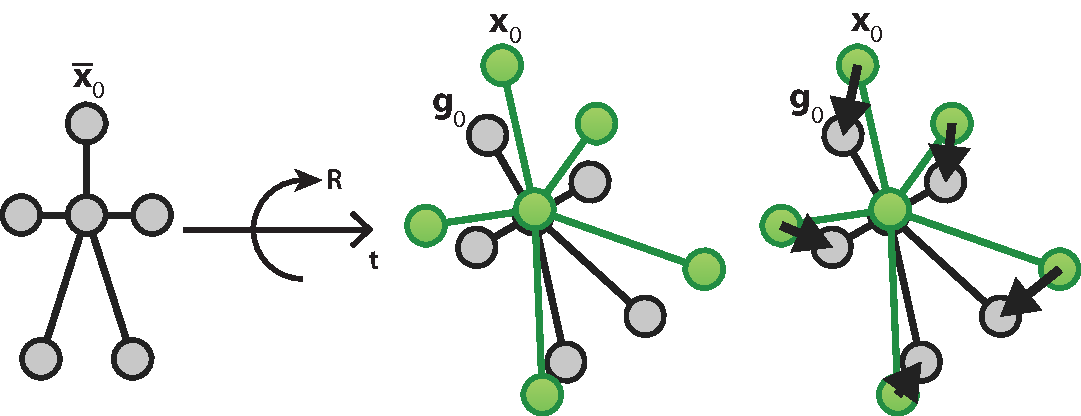
\includegraphics[width=.96\textwidth]{images/shape_matching.pdf}
\caption{Shape matching illustration}
\label{img:shape_matching}
\end{figure}

The algorithm only takes a set of particles and there initial configuration as inputs. Each particle has four variables

\begin{align*}
m_i &, \text{the mass} \\
\bar{x}_i &, \text{the rest position} \\
x_i &, \text{the current position} \\
v_i &, \text{the velocity}
\end{align*}

The integration scheme uses the goal positions \(g_i\) to move the particles to the desired goal positions. The amount of movement can be directly modeled as a simple stiffness parameter \(\alpha\). A stiffness parameter if \(1\) thus basically doesn't allow for any deformation as the particles are always moved to their ideal transformed state. By using all these information and the external forces (i.e. gravity) the integration step becomes:

\begin{align}
v_i(t+h) &= v_i(t) + \alpha * \frac{g_i(t)-x_i(t)}{h} + h * f_{ext}(t)/m_i \\
x_i(t=h) &= x_i(t) + h * v_i(t+h)
\end{align}

The goal position \(g_i\) is obtained by shape matching the rest shape to the current deformed shape. The problem shape matching solves is thus defined by finding the rotation matrix \(R\) and the translation vector \(t\) between the two sets of points \(\bar{x}_i\) and \(x_i\). The desired matrix \(R\) and vector \(t\) minimize the following term:

\begin{equation}
\sum\limits_i m_i(R(\bar{x}_i-\bar{t})+t-x_i)^2
\label{eq:minimize_shape_matching}
\end{equation}

The optimal translation vectors are simply the respective center of masses of the rest shape and the deformed shape.

\begin{equation}
\bar{t} = \bar{c} = \frac{\sum_{i} m_i \bar{x}_i}{\sum_{i}m_i}, t = c = \frac{\sum_{i} m_i x_i}{\sum_{i}m_i}
\end{equation}

Unfortunately the optimal rotation matrix is not as simple to compute. The equation \ref{eq:eq:minimize_shape_matching} has to be simplified. The first step is to define relative positions for all points with respect to their center of mass.

\begin{gather}
q_i = \bar{x}_i - \bar{c}, p_i = x_i - c \\
\sum\limits_i m_i(Rq_i-p_i)^2
\label{eq:center_of_mass_shape_matching}
\end{gather}

The next insight is to actually find the optimal linear transformation \(A\) instead of the optimal rotation matrix \(R\).  Calculating the derivative with respect to all coefficients of \(A\) and setting it to zero gives the optimal linear transformation.

\begin{equation}
A = (\sum_i m_i p_i q_i^\top)(\sum_i m_i q_i q_i^\top)^{-1}=A_{pq}A_{qq}
\end{equation}

\(A_{qq}\) is a symmetric matrix can therefore contains no rotational part. All the rotation is encapsulated in \(A_{pp}\). The optimal rotation matrix can now be found by calculating the polar decomposition \(A = RS\). This allows to finally write down the goal position for each particle as

\begin{equation}
g_i = R(\bar{x}_i - \bar{c}) + c
\end{equation}

All particles are than moved to their respective goal positions by a variable fraction. This fraction effectively models the stiffness of the deformable body. If the stiffness fraction is close to $1$ the particle practically snap to their ideal goal positions which by definition are not deformed as they only include translation and rotations of initial rest state. If the stiffness fraction on the other hand is very low the particles stay in their predicted position and bodies is completely deformed.

\section{Position Based Dynamics}
\label{sec:position_based_dynamics}

Position based dynamics is a method which omits the traditional force based approach simulate dynamics systems but instead directly works on the positions to simulate deformable objects. This means it also is not physically correct but instead provides an efficient unconditionally stable simulation. Like shape matching it also tries to satisfy constraints in order to arrive at stable end positions. But instead of one global constraint, the shape, position based dynamics handles many different constraints. These constraints either model the physical properties of the object and are thus fixed throughout the simulation, or are generated on demand in the case of collision constraints used to resolve collisions. Also as the name implies position based dynamics only works with the position of the particles updating them directly. The velocity of the particle is solely determined by the difference in positions overtime. This is best illustrated by the the pseudocode of the simulation loop.

\begin{algorithm}[htbp]
\caption{Position based dynamics simuation}
\begin{algorithmic}[1]
\FORALL{vertices $i$}
	\STATE{initalize $x_i=\bar{x}_i, v_i =\bar{v}_i, w_i = 1/m_i$}
\ENDFOR
\LOOP
	\FORALL{vertices $i$} \STATE{$v_i \gets v_i + \Delta t w_i f_{ext}(x_i)$}\ENDFOR
	\STATE{dampVelocities($v_1,...,v_N$)}
	\FORALL{vertices $i$} \STATE{$p_i \gets x_i + \Delta t v_i$}\ENDFOR
	\FORALL{vertices $i$} \STATE{generateCollisionConstraints$(x_i\rightarrow p_i)$} \ENDFOR
	\WHILE{$i \leq solverIterations$}
		\STATE{projectConstraints$(C_1,...,C_{M+M_{coll}},p_1,...,p_N)$}
	\ENDWHILE
	\FORALL{vertices $i$} 
		\STATE{$v_i \gets (p_i-x_i)/\Delta t$}
		\STATE{$x_i \gets p_i$}
	\ENDFOR
	\STATE{velocityUpdate$(v_1,...,v_N)$}
\ENDLOOP
\end{algorithmic}
\end{algorithm}

The first key insight into the algorithm occurs in lines 9-11. Here positions for all vertices are estimated using the current velocity and the time step. This step is completely unrestricted and just predicts and estimates a position which is then later redefined. Line 15-17 illustrate this refinement. A Gauss-Seidel type iteration is used to satisfy all constraints defined for the system. These constraints mostly model the inherent structure of object currently simulated but another important aspect handled here are collisions with are just another constraint for the system and generated in each time step after estimating the position. The idea is to iterate over all constraints multiple times so that the particles are projected to valid locations with respect to the given constraint. The final vital piece of the algorithm can be seen in lines 18-21. After all constraints have been satisfied as best as possible the estimated positions alone are used to update the state of all vertices. The velocity of the particle is solely calculated by the difference of the new estimated position and the former position. This integration scheme is unconditionally stable as it doesn't just extrapolate into the future like traditional explicit schemes do. Instead it uses the physically valid positions computed with the constraint solver.

\section{Oriented Particles}
\label{sec:oriented_particles}

Oriented particles combines the geometrical based approach of shape matching with the idea of updating the velocities based on the positions alone as described in position based dynamics. The specifically improves upon shape matching in sparse regions increasing the overall stability of the shape matching. Modeling the particles as oriented ellipsoids can approximate the surface more accurately than simple sphere which is especially useful in calculating and resolving collisions.

\subsection{Generalized Shape Matching}
The main idea is to use oriented particles that in addition to the position and velocity also store rotation and spin. The particles now all have orientation information associated with them, thus the name of the method. The variables for each particle thus are now extended to encompass the following seven variables.

\begin{align*}
m_i &, \text{the mass} \\
\bar{x}_i &, \text{the rest position} \\
\bar{q}_i &, \text{the rest orientation} \\
x_i &, \text{the current position} \\
q_i &, \text{the current orientation} \\
v_i &, \text{the linear velocity} \\
\omega_i &, \text{the angular velocity}
\end{align*}

The advantages to include orientations for each particle become particular evident in sparse regions of the model like for example chains of particles or even single particles. The traditional approach of using spherical particles to model twisting chains would involve adding many particles to capture the twist. In order to model the same scenario with oriented particles only a single particle is required as the twisting is completely captured in the rotation and spin of the particle.

\begin{figure}[htbp]
\centering
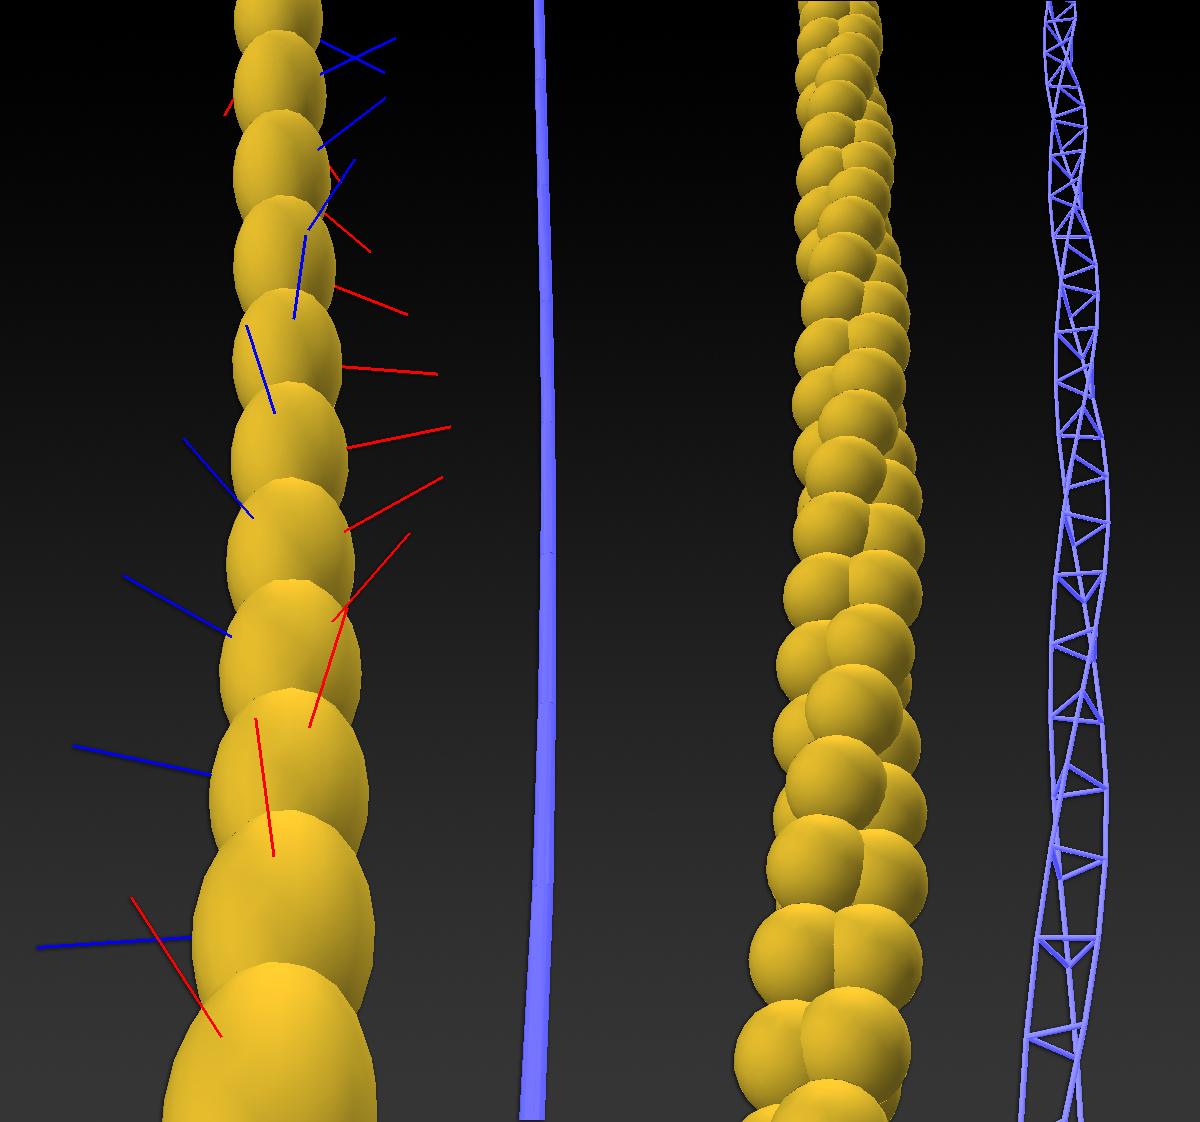
\includegraphics[width=.5\textwidth]{images/oriented_particle_twist_chain.png}
\caption{Oriented particle twisting chain}
\label{img:rigid_body}
\end{figure}

The basic approach of shape matching is directly applied to the generalized shape matching used for the oriented particle but differs in the way the moment matrix is calculated. The original minimization function \ref{eq:minimize_shape_matching} is slightly modified so it becomes the following moment matrix $A$, but is essentially still the same as in the original shape matching approach.

\begin{equation}
A = \sum\limits_i^n m_i(x_i-c)(\bar{x}_i - \bar{c})^\top  \in \mathbb{R}^{3x3}
\label{eq:minimize_oriented_particle}
\end{equation}

This moment matrix $A$ in terms of $n$ particles each with a corresponding mass $m_i$ and current position $x_i$. The center of mass for the current configuration is defined as $c$. Analog to that the rest position is defined as $\bar{x}_i$ and the rest center of mass as $\bar{c}$. Both center of mass are calculated using the traditional approach as seen in equation \ref{eq:center_of_mass_shape_matching}.

As in the original shape matching the goal is to find the optimal translation vector $t$ and rotation matrix $R$, which map the original shape to the current configuration in a least squares manner. The optimal translation vector can simply be calculated from the differences of the two centers of mass.

\[
t = c - \bar{c}
\]

The rotation matrix $R$ can be obtained by calculating the polar decomposition of $A$

\[
A = R*S
\]

Together with translation vector $t$ and the extracted rotation matrix $R$ the goal positions for each particle can be calculated.

\[
g_i = R(\bar{x}_i-\bar{c})+c
\]

Thus far this is still exactly the same as in the original shape matching approach. Unfortunately  the moment matrix $A$ can become ill-conditioned are even singular. This happens if the particle are close to co-planar or as in the example of the twisting chain co-linear. If $A$ is ill-conditioned the polar decomposition is not well defined and yields only unusable and unstable results. Thus no reliable $R$ can be obtained. Adding the orientation information for each particle into the calculation can fix this problem.

The solution involves defining a well-conditioned moment matrix for even single particle and consequently adding each moment matrix together in order to arrive at a total moment matrix for the whole particle group. In order to arrive at this result lets begin with two groups of particles, each with their own unknown moment matrix $A_1$ and $A_2$ respectively. Both moment matrices are defined with respect to their own center of mass and thus can not simply be added to arrive at the combined moment matrix. As described in Rivers and James equation \ref{eq:minimize_oriented_particle} can be reformulated to the following formula which shifts the center of mass to the global one.

\begin{equation}
A = \sum\limits_i^n m_ix_i\bar{x}_i^\top - Mc\bar{c}^\top
\label{eq:minimize_oriented_particle}
\end{equation}

Here $M$ is simply defined as the sum of all particle masses. Now the next step is to apply the same logic to each individual particle forming the group instead of two separate groups. This yields the following equation

\begin{equation}
A = \sum\limits_i^n (A_i + m_ix_i\bar{x}_i^\top-m_ic\bar{c}^\top)
\end{equation}

$A_i$ denotes the moment matrix for a single particle in the group while the other variables retain their original meaning. This equation can be generalized and improved further.

\begin{equation}
A = \sum\limits_i^n (A_i + m_ix_i\bar{x}_i^\top) - Mc\bar{c}^\top
\end{equation}

Integrating the equation \ref{eq:minimize_oriented_particle} over the particle's volume yields the moment matrix for a single particle. Each particle is modeled as an ellipsoid so their moment matrix is defined in terms of their radii and rotation.

\begin{equation}
A_{\text{ellipsoid}} = \frac{1}{5}m \begin{bmatrix} a^2 & 0 & 0 \\ 0 & b^2 & 0 \\ 0 & 0 & c^2  \end{bmatrix} R
\end{equation}

The radii of a single particle are simply defined by the length of the semi-axes $r = [a,b,c]^\top$ in all orthonormal directions. Including the orientation $R$ for each single particle causes the total moment matrix $A$ to always be full ranked and thus the polar decomposition to return more reliable results.

Having defined a stable moment matrix for each group the optimal translation vector and rotation matrix can be obtained and thus the goal positions can be calculated. Again analog to the original shape matching the particles are pulled towards their goal positions by a variable stiffness fraction. However the oriented particles way of integrating the position and velocities of the particles is completely different from the way the traditional shape matching method works. Instead the oriented particles are update and integrated by a system closely modeled after the position based dynamics approach but extended by integrating the orientations of the particles.

\subsection{Generalized Position Based Dynamics}
As in PBD the first step is the prediction step. Here a new predicted position $x_p$ is calculated for each particle using a simple integration scheme. However for oriented particles the associated orientation $q_p$ of each particle has also to be predicted over time. This prediction step using an explicit euler integration looks like the following.

\begin{align}
x_p &\leftarrow x + v\Delta t \\
q_p &\leftarrow [\frac{\omega}{|\omega|}sin(\frac{|\omega|\Delta t}{2}), cos(\frac{|\omega|\Delta t}{2})]q
\end{align}

Now the solver has calculated a predicated state $(x_p,q_p)$ for each single particle. This information is then based onto the second step. The second step is simply the adaptation and modification of the predicted state according to the rules laid out by the generalized shape matching approach outlined above. The last and final step integrating the state for each particle. In accordance with PBD but in difference to shape matching the integration step only takes in the particle's state in the beginning of the iteration and the adjusted predicted state. This way, like in PBD, of calulating the velocities solely based on the positions and orientations provides an unconditionally stable scheme as the adjusted predictions never overshoot. The integration step thus becomes the following equations.

\begin{align}
v &\leftarrow (x_p - x)/\Delta t \\
x &\leftarrow x_p \\
\omega &\leftarrow axis(q_p q^{-1}) \cdot angle(q_p q^-1)/\Delta t \\
q &\leftarrow q_p
\end{align}

The function $axis(q)$ simply returns the normalized direction of the quaternion $q$ and $angle(q)$ consequently the angle. One caveat to take note of is the observation that there are always two possible rotations $r=q_pq^{-1}$ to transform $q$ into $q_p$. It is important to choose the smaller rotation of the two to update the angular velocity $\omega$.

The standard simulation model for oriented particles uses an implicit shape matching. For implicit shape matching the particle belonging to an implicit shape matching group are defined by their edges. A group exists for every particle at the center and additional all the particles connected to this center particle by an edge. This results of this usually look like a tetrahedral mesh in more connected regions and thin particle chains in very sparse regions. However the topology of the particles can be completely arbitrary.

In practice a Gauss-Seidel type iteration scheme is used to satisfy all shape matching constraints defined by the implicit groups. This reduces the effect of the inherent bias towards the first groups that are evaluated during the execution. After updating the predicted state multiple times taking into account all groups the predicted position of each particle is moved towards the calculated goal position by a stiffness fraction. The orientation on the other hand is only updated for the respective center particle.

\subsection{Collision Handling}
\label{subsec:collision_handling}

Another improvement oriented particles provide is a more accurate collision handling. Each oriented particle is no longer a simple sphere but instead is modeled as an ellipsoid.

\begin{figure}[htbp]
  \centering
  \subfigure[Sphere collision]{
      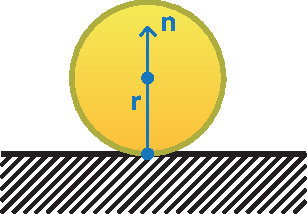
\includegraphics[width=.3\textwidth]{images/oriented_particles_collision_sphere.pdf}
     \label{subfig:collision_sphere}
  }
  \subfigure[Incorrect ellipsoid collision]{
      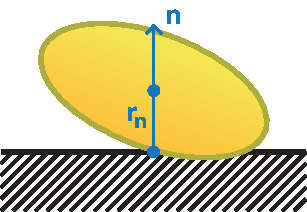
\includegraphics[width=.3\textwidth]{images/oriented_particles_collision_ellipsoid_wrong.pdf}
     \label{subfig:collision_ellipsoid_incorrect}
  }
  \subfigure[Correct ellipsoid collision]{
      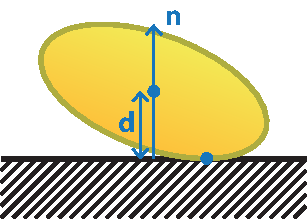
\includegraphics[width=.3\textwidth]{oriented_particles_collision_ellipsoid_correct.pdf}
     \label{subfig:collision_ellipsoid_correct}
  }
  \label{fig:collision_handling}
\end{figure}

Ellipsoids can fit better to the surface area of a model than simplistic spheres. Using sphere might cause unnatural frictions or other visual artifacts. The question now remains how to calculate the correct spot on the surface of the ellipsoid that collided with a plane as can be seen in figure \ref{subfig:collision_ellipsoid_correct}. The simplistic approach used in the spherical case can not be directly transferred as illustrated in figure \ref{subfig:collision_sphere} and \ref{subfig:collision_ellipsoid_incorrect}. This would only work if the contact normal is aligned to the principal axis of the ellipsoid. However, in almost all cases this is not the case and the calculation becomes a little bit more involved.

Each potential particle is defined by its principal radii $a,b,c$ and its rotation matrix $R$. The potential collision plane is simply defined in hessian form as $p = n^\top x=d$. The first step is to compute the contact point on the surface of the ellipsoid with a normal that is parallel to the normal of the plane $n$. In general the ellipsoid can be defined in terms of the following zero iso-surface.

\begin{equation}
c(x) = x^\top A x - 1
\end{equation}

The potential contact point has to meet the following two constraints

\begin{align}
\nabla c(x)&=\lambda n \\
c(x) &= 0
\end{align}

In addition to these two constraints the following two formulas yield enough information to solve for $\lambda$ and $x$, though only $x$ is of real interest.

\begin{align}
\nabla c(x)&=2 A x \\
A = R \begin{bmatrix}\frac{1}{a^2} & 0 & 0 \\ 0 & \frac{1}{b^2} & 0 \\ 0 & 0 & \frac{1}{c^2}\end{bmatrix} R^\top &\Rightarrow A^{-1} = R \begin{bmatrix}a^2 & 0 & 0 \\ 0 & b^2 & 0 \\ 0 & 0 & c^2\end{bmatrix}R^\top
\end{align}

Thus $\lambda$ and $x$ can be calculated in the following manner.

\begin{align}
\lambda &= \pm \frac{2}{\sqrt{n^\top A^{-1} n}} \\
x &= \pm \frac{A^{-1}n}{\sqrt{n^\top A^{-1} n}}
\end{align}

These calculations always lead to two possible positions $x$ on the surface of ellipsoid with have a normal to the plane normal. The correct point to choose is always the point which is closer the plane, this can be easily calculated given the hessian form of the plane. The final step to determine if a collision between the current particle and the plane has occurred is to check if the contact point is below the plane and thus satisfies the condition $n^\top x < d$. Solving this condition also automatically returns the penetration depth of the collision. The depth can be directly utilized to modify the predicted position of particle. The collision detection and resolution step is done for all particles after the positions have been predicted but before the shape matching. Although the collision step should ideally be calculated for every iteration, using Gauss-Seidel, of the shape matching, this is way to expensive as the number of particles and planes can get quite large very quickly. However, just resolving the collisions once before shape matching seems to give satisfactory results.

The oriented particles paper describes a couple of additional features for the simulation with oriented particles. These include explicit shape matching groups defined manually, plastic deformation which cause the rest state to change, friction, torsion resistance, stretching and bending, collision handling between two ellipsoids and using the orientation information for more efficient skinning. However, these features are not needed to achieve the goals and requirements of this thesis and are thus not described here. More details can be found in the original paper.
\chapter{Conceptual Approach}
\label{cha:conceptual_approach}

The simulation tries to combine a traditional rigid body simulation with the simulation of deformable bodies using oriented particles. The idea is to have an object which consists of both a rigid core and a surrounding soft layer. Both these layers will be simulated using their respective dynamics system. Both the interaction of such a combined body with the world as well as the interaction between the two layers is explained using the proposed technique.

\section{Simulation Model}
\label{sec:simulation_model}

Every object in the simulation is either a combined body or a simple rigid body. The simulation model describes how these different bodies are modeled and constructed in order to enable the simulation and interaction between them. This requires both a model for rigid bodies as their used both alone as well as at the core of the combined body. Oriented particles are used for the deformable parts. Combining these two models into a unified combined body is the main contribution of this thesis.
\subsection{Rigid Body}

Simple rigid bodies are used to simulate objects which do not have or do not need a soft surrounding layer. Most prominently the object being picked up is for simplicity's sake a simple rigid body. Also the ground does not need to be deformable and is thus simulated as a rigid body. These usually static rigid bodies are simulated using the traditional rigid body dynamics. They have all the usual properties of rigid bodies. The position, orientation, linear velocity and angular velocities are simulated over time. External forces, like gravity, act on the bodies and cause a change in velocity. The velocities are then updated in the collision resolution step using impulses. Finally the position and orientation are integrated and updated.

\subsection{Oriented Particles}

The oriented particles form the deformable tissue of every combined body. They are simulated exactly like the proposed by Mueller et al.. All particles have position and velocity. After updating the velocities shape matching is used to arrive at an optimal configuration of the deformed particles. The position of the particles are then moved towards this configuration. In the final step new velocities are calculated for each particle based solely on the new position of the particle.

\subsection{Combined Body}
\label{subsec:combined_body}
Combined bodies are more complex. These bodies are a combination of a rigid inner core with a soft outer shell. The rigid inner body behaves exactly like a traditional rigid body or other non-combined bodies in the simulation. For each combined body a number of variables have to be maintained. First for the inner core the same variables as for any other rigid body are needed. These are the positions of the center of mass, the orientation, the linear velocity and the angular velocity. The particles building up the soft tissue have the same variables as original oriented particles, meaning rest position, current position, rest orientation, orientation, linear velocity and angular velocity.

There are two general types of forces acting on the combined body. The first are external force, most prominently gravity. The second ones are internal forces occurring at the interface between the inner core and the outer tissue. External force are only applied to the inner rigid body, while the resulting changes in the tissue are simply the result of the inner force propagation. How exactly force propagation is implemented will be discussed in section \ref{subsec:force_propagation}. Another source of changes of the state of the body are collisions which will be described in detail in section \ref{subsec:theory_collision_handling}.

The particles of the deformable tissue are divided into two types. The first type is called attached particle. Attached particles are evenly distributed across the surface of the inner core. They provide the interface between the outer tissue and the inner bone. These particles are glued to the rigid body and provide the means to have force propagation from the particles to the core if the tissue or inner core are moved relative to each other.

The second type of particles are simply called outer particles. The outer particles are used to model the shape and structure of the surrounding tissue. They can be positioned and arranged in any desirable way. The simulation places no limitations on the shape of the outer tissue. The only obvious requirement is that the outer particles are well connected to the layer of the attached particles on the surface of the rigid core, as otherwise the tissue could simply separate from the bone.

All particles, regardless if attached or outer particle, are simulated according to the approach described in the oriented particles paper, no modifications are needed. This also holds true for the shape matching constraints, which are defined implicitly. However the simulation again does not place any limitations on the way connections are modeled.

\subsection{Collision Handling}
\label{subsec:theory_collision_handling}

There are three different types of collisions handled by the current simulation model.

\begin{enumerate}
\item Rigid Body $\leftrightarrow$ Rigid Body
\item Combined Body $\leftrightarrow$ Rigid Body
\item Outer Tissue $\leftrightarrow$ Inner Bone
\end{enumerate}

The first type of collision between two rigid bodies is handled in the traditional way. For each pair of rigid bodies a set of contact points is calculated when they collide. Taking into account the velocities of both bodies at each contact point and the resulting relative velocity the collision is resolved using impulses. The impulses cause an immediate change in velocity for each body. Both the resulting normal force separating the two bodies and the friction force are taken into account.

The second type of collision occurs between a combined body and a rigid body. Actually this type of collision is divided into many subcollision checks comparing the particles with the planes of the rigid body. The subcollisions are only evaluated with regard to the outer particles. This is motivated by the assumption that the tissue can never be compressed to such a degree that the attached particle could ever come into contact with the outer world. For each outer particle the contact points are calculated, taking advantage of the ellipsoid shape of the particles. This happens in exactly the same way as described in the original oriented particles paper, with the addition to having to compare every outer particle with every face of the rigid body. 

However, the collision resolution cannot directly be applied to the rigid body. The simulation model proposes a novel hybrid approach, combining the position based approach for particles with an impulse based approach for the rigid body. The collision response for the particle is exactly the same as for the general case. The penetration depth of the particle is calculated and the predicted position of the particle is simply moved out of the rigid body along the contact normal.

The effect on the rigid body however is calculated using the traditional rigid body simulation. The exact same algorithm used for rigid and rigid collisions is employed. The colliding particle is simply interpreted as a rigid body and fed to the exact same algorithm used for rigid-to-rigid body collisions. The resulting force is therefore both calculated for normal direction as well as for friction. However, these forces are only applied to the rigid body and not to the particle. This approach of course is not physically correct, but yields satisfactory and plausible results.

The third type of collisions between the outer soft tissue and the inner rigid bone of each combined body is modeled in a similar way to the approach taking in Position Based Dynamics. This approach and the application to the combined body is discussed in section \ref{subsec:force_propagation}. Another theoretical possible collision type not mentioned thus far is between two combined bodies, which comes down to collisions between particles. This type of collision is not modeled in the current simulation model, as it lies outside the requirements.

\subsection{Force Propagation}
\label{subsec:force_propagation}

Force propagation defines and models the forces occurring between the outer soft tissue and inner rigid bone. During the simulation the surrounding tissue and the inner core will move relative to each other, which will have to be corrected as otherwise the two parts would simply separate. The approach is modeled in a similar manner to the way Position Based Dynamics models the collision of particles with rigid bodies. The impulse used in PBD is calculated using the following formula.

\begin{equation}
J = m_i \Delta p_i/\Delta t
\end{equation}

This impulse is applied to the rigid body at the contact point in case there was a collision. However, for  the inner force of a combined body the problem is not that simple. In case of the combined body only the attached particles have to be evaluated, again under the assumption that the tissue cannot be deformed enough to cause the outer particles to collide with the inner core. After all shape matching iterations have finished the attached particles have a final predicted position. However, this position is most likely not on the surface of the inner rigid body. They either end up inside the core or further away. The case of being inside is exactly the same as the collision case described in PBD which results in a push force on the rigid body. The case of settling away from the surface, however should also result in a force, more specifically the core should be pulled towards the attached particle. In order to calculate the correct impulse for both cases the attached particles are realigned to their position on the surface, which causes a response in the rigid body. Calculating the correct impulse first requires $\Delta p_i$, which can be obtained by comparing the current predicted position $x_p$ with the rest position $x_r$ on the surface of the core relative to the core's current transformation in world space $T$.

\begin{align}
x_r &= T\bar{x}_r \\
\Delta p_i &= x_p - x_r
\end{align}

Here $\bar{x}_r$ denotes the relative position of the particle relative to the resting transform of the cube. The resulting impulse is then directly applied to the $x_r$ on the body. In the final step the predicted position of all attached particles is forcefully set to $x_r$, so that they appear glued to the surface of the inner rigid core.

\section{Requirements}

In chapter \ref{cha:problem_analysis} a number of main requirements were defined. All of these requirements can now be compared and validated against the proposed simulation model, as described in chapter \ref{cha:conceptual_approach}.

\paragraph{1. Real-time Simulation}

As arguably the most important requirement, the real time aspect of the overall simulation directly depends on the performance of the individual subsimulations. The system includes a complete, although simplistic, rigid body simulation. Rigid body simulations are relatively straightforward and have been around for a long time. A huge number of bodies can be simulated reliable and in real time. So this subcomponent meets the requirement implicitly. The other subcomponent is a direct application of the concepts introduced by the oriented particles' paper. The goal of that paper was also the real time applicability of the deformable simulation. The authors proved this important characteristic quite successfully. So another component passes the requirement implicitly. 

The two major additions are the collision resolution between outer particles and rigid bodies and the force propagation inside the combined body. The force propagation is of linear complexity and has to only be calculated for a rather limited number of attached particles. Thus it doesn't have any significant impact on the real time requirement.

The collision resolution involving the outer particles is the most computationally intensive component. Each particle has to be compared against to every face of the rigid body. Fortunately this can basically be reduced to a collision detection between two rigid bodies with all possible optimizations. The calculations are in fact even easier than that because the particles are perfect ellipsoids, which reduces the required comparisons significantly.

All components contributing to the overall simulation are capable of real time. Thus the overall simulation will run in real-time and the requirement is fulfilled.

\paragraph{2. Low Number of Bodies}

The first step in reducing the number of bodies in the simulation was already taken by the oriented particles approach, which allows to simulate fewer particles overall and especially in sparse regions. By using the rigid core for the combined body the number of particles can be further reduced as the internal structure no longer has to be modeled using particles. In practice these inner particles might not even be deformed at all as the external forces are not large enough and are thus needlessly consume resources. Using the soft surrounding layer enables the tissue to wrap around the other object. This increases the contact area between the two bodies and reduces the need to model the same scenario with multiple rigid bodies connected by joints.

\paragraph{3. Only Approximate Orientation of Finger Relative to Object}

By enabling the soft tissue to wrap and deform around other objects the contact area between the bodies is increased which allows for more stable simulations. Using rigid bodies for the same tasks can result in numerical instabilities because of the way collisions are detected and resolved. This goes especially for completely non-trivial shapes where because of the rasterization the perfect solutions cannot always be found. The deformable tissue solves this as it can smooth out these instabilities over time.

\paragraph{4. Force Propagation Inside Body Between Tissue and Bone}

The force propagation inside the body is explicitly modeled and described in section \ref{subsec:force_propagation}. Permanently attached particles on the surface of the bone propagate the forces resulting from changes of the surrounding tissue. Thus the tissue is always firmly glued to the bone and nothing can drift apart.

\paragraph{5. Friction Between Finger and Object}

The ways forces are handled between oriented particles and rigid bodies are explicitly modeled and described in section \ref{subsec:collision_handling}. Friction is only acting on the rigid body but not on the particles. Although this is not at all physically correct it behaves plausible and believable.

\chapter{Solution Details}
\label{cha:solution_details}

The proposed simulation framework is implemented in a small proof of concept application. The application provides a simple playground to test, evaluate and demo various scenes. The provided application was only developed and tested under MacOS X Lion, but the small number of required dependencies are all available as cross-platform libraries for Windows, MacOS X and Linux. 

The application was written in the C++ programming language because it is the predominate language in the area of physical simulations and for the easy integration with dependencies. The graphics pipeline runs on OpenGL and to simplify its usage the OpenGL Utility Toolkit (GLUT) was also heavily used. The only other major dependency is the Bullet Physics Library (Bullet).

Bullet is almost exclusively used to handle and manage the rigid bodies in the scene. This includes integrating velocities and positions as well as handling collision detection and resolution for rigid body to rigid body collisions. Bullet is not used deliberately for the collision detection and responses between rigid bodies and oriented particles. Both the external collisions as well as the inner force propagations are implemented in their respective collision handlers. This allows for the necessary customizations to implement the proposed algorithms.

Bullet's built in linear math module is used throughout the code for the various mathematical formulas and provides the basic vector and matrix primitives. This includes all the code required to implement the deformable parts of the simulation. Every oriented particle, their simulation and their collisions are calculated using the provided math functions. However, apart from these functions the code for the oriented particles and custom collision handlers is completely hand-written. This is also the reason why the performance of these code sections is not ideal. The focus of the current implementation is solely a proof of concept and only meant to allow for general and simple comparisons.

\section{Code Structure}

The complete implementation requires only four classes. The main application function only sets up the graphics context including to navigate the scene with the keyboard and runs the main execution loop for the simulation.

\paragraph{Simulation Class}
The Simulation class implements everything required for setting up the concrete scene and handles each simulation step. The simulation class also implements all collision code. The collisions between purely rigid bodies are handed of to bullet for detection and the resolution is then manually calculated inside the simulation class. For oriented particles the code for the collision detection and resolution is entirely implemented inside the class itself in order to provide maximum customization.

Currently the scenes always consist of a ground and a variably sized block which will be the object to be picked up. The ground is a simple static rigid body and does not move or react to forces during the entire simulation. The block is also a rigid body but it is completely alive. This means both gravity and later the pickup forces act and modify the state of the block. The block can both have an arbitrary size and mass.

To either side of the block two fingers are positioned. These fingers can either be completely rigid or be the new combined bodies consisting of both a rigid inner bone and a soft outer tissue. If the fingers are rigid their simulated exactly the same as any other rigid body with the help of the bullet library. Combined bodies are simulated using the custom CombinedBody class with will be described later.

For simulation purposes the force and resulting velocities are set manually for the two finger, regardless if they are rigid bodies or combined bodies. This is done to simulate fixed fingers which can not be pushed apart and are exert a constant push force as well as a constant force upwards. In order to facilitate this property the linear velocity in x is capped at zero for both pushing directions, this means the left finger is only allowed to push into the positive direction and has a minimum velocity in x of zero. The right finger on the other hand is only allowed to push into the negative direction and has a minimum maximum velocity of zero. In velocity in y is not capped as it will always point upwards, however both fingers velocity in y is synchronized so that one finger can't move faster than the other. The velocity in z as well as the angular velocity is always set to zero so no movement can occur. These modifications are necessary for the current simple simulation only, in an improved version controllers and motors would be needed to more realistically model somewhat fixed and stable fingers.

\paragraph{CombinedBody Class}
The CombinedBody class holds all the information required for the proposed two part body consisting of an inner rigid bone and outer soft tissue. The rigid part is built using the btRigidBody class provided by the bullet library. For the deformable part multiple instances of the custom class ParticleGroup is maintained. The CombinedBody class handles the states for the rigid body and all particles and provides basic functions to apply forces and integrate the velocities and positions.

One major functionality integrated into the CombinedBody class is the initialization of the soft outer tissue. Also the structure of the oriented particles is in the tissue is arbitrary as far as the simulation is concerned a concrete sample implementation is provided. The underlying geometric structure chosen relies on an evenly distributed number of so called attached particles across the surface of the inner rigid body. Currently only a version for box-like shaped bodies is provided. The layout algorithm for the attached particles starts by iterating over all faces of the box. An attached particles is added for each corner. Then depending on a customizable density parameter additional particles are added to each edge. Finally the rest of the face is filled according to the grid defined by the particles on the corners and edges. An illustration of this can be seen in figure \ref{fig:combined_body_density}.

\begin{figure}[htbp]
  \centering
  \subfigure[$density = 1$]{
      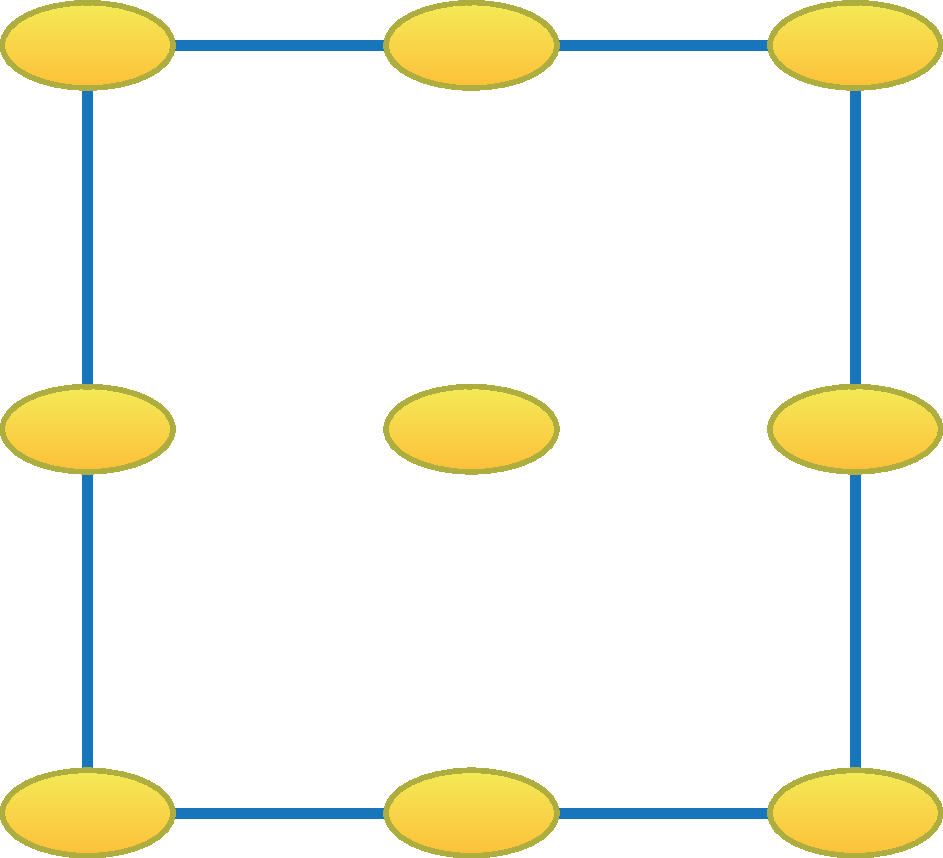
\includegraphics[width=.3\textwidth]{images/combined_body_density_1.pdf}
     \label{subfig:combined_body_density_1}
  }
\hspace{2cm}
  \subfigure[$density = 2$]{
      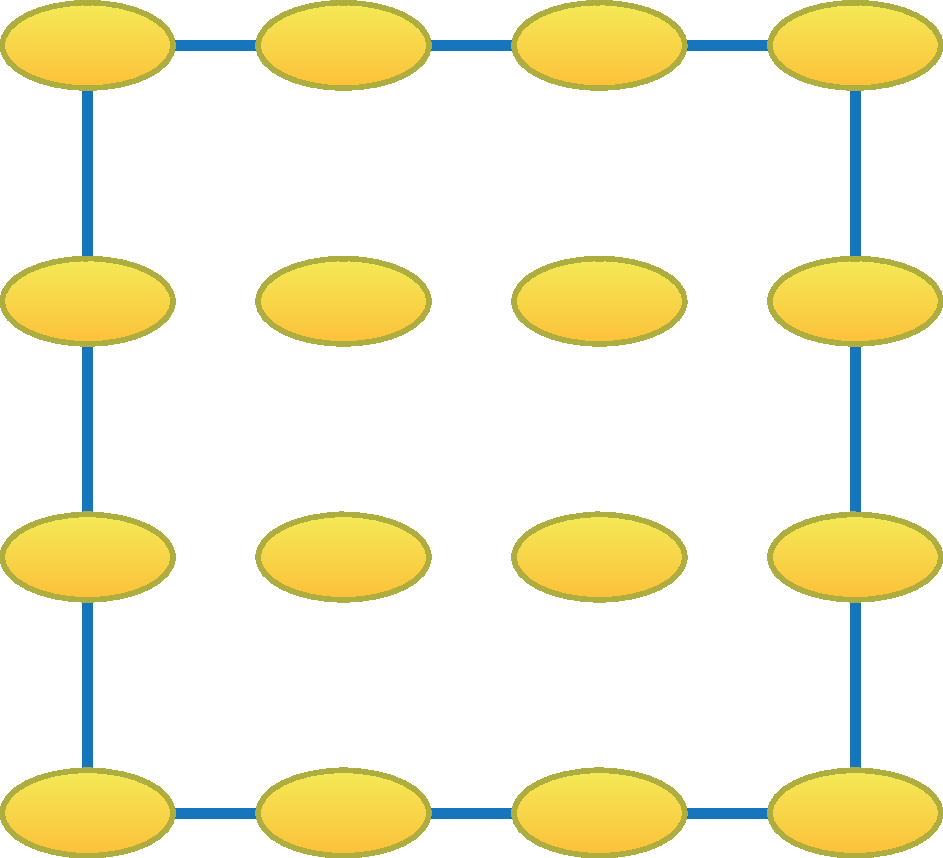
\includegraphics[width=.3\textwidth]{images/combined_body_density_2.pdf}
     \label{subfig:combined_body_density_2}
  }
  \label{fig:combined_body_density}
\end{figure}

For the outer soft tissue the inner attached particles are simply extrude by a configurable factor from the center of mass of the inner core. This results in a simple one layer outer layer. Again the simulation itself does not place any restrictions on the structure of the tissue, but this simple algorithm proved to be sufficient. The last step required to a complete model of the deformable outer part is generating the implicit particle groups required for shape matching.

The concrete algorithm to accomplish this is not really important, only two restrictions have to be taken care of. First a high enough degree of interconnectiveness must be ensured. In the original oriented particles paper the implicit connection is simply taken from the underlying mesh of vertices connected by the edges. The second restriction is that the outer particles have to be connected to the attached particles on the surface, as otherwise the skin would just come off.

The current implementation currently iterates over all particles on each respective layer(attached and outer). For each particle $p$ a list of all particles in the current layer is generated and sorted by the distance to particle $p$. This ensures that the particle itself is always at index $0$ of this list, followed by its closest neighbors. A configurable number $n = groupSize$ of particles taken from the beginning of this list is than added to a particle group with the particle $p$ at the center. At last the corresponding particle in the other layer is also added with the help of the extrude factor, ensuring the connection of both layers. So every group in the end consists of $n = groupSize + 1$ particles. This is done for both the attached particle layer as well as the outer particle layer in order to generate all the particle groups required for shape matching.

\paragraph{ParticleGroup Class}
The ParticleGroup class holds all particles belonging to a specific implicit shape matching group. It implements all the functionality required to execute the shape matching algorithm. This includes calculating the current center of mass and the moment matrix across all particles. The polar decomposition is also implemented here. The implementation adapted from Higham \ref{??} as it is implemented in the bullet library\footnote{\text{http://bulletphysics.com/Bullet/BulletFull/btSoftBodyInternals\_8h\_source.html}}. Using all these subcomponents in the final calculation of the goal positions and subsequent adjustment of the predicted position is also the responsibility of the particle group.

\paragraph{Particle}
The Particle class holds all the required state variables for an oriented particles as described in section \ref{sec:oriented_particles}. This also includes all derived and intermediary variables. Both the predicted position and orientation of the particle are maintained here as well as the current moment matrix for a single particle.

\section{Loop}

This section illustrates the simulation step executed for each time step. It only shows the loop as it is implemented for the deformable scenario. The scenario with only rigid bodies is essentially identical to the sample loop provided in section \ref{sec:rigid_body_simulations} about rigid body simulations.

\begin{algorithm}[htbp!]
\caption{Combined Body Simulation Loop}
\begin{algorithmic}[1]
\FORALL{bodies $b_{all}$}
	\STATE{apply gravity}
	\STATE{integrate velocity}
	\STATE{predict state}
\ENDFOR
\FORALL{fingers $f$}
	\FORALL{outer particles $p_{outer}$}
		\STATE{resolve collision with ground}
	\ENDFOR
	\FORALL{outer particles $p_{outer}$}
		\STATE{resolve collision with block}	
	\ENDFOR
\ENDFOR
\FORALL{gauss-seidel iterations $i$}
	\FORALL{fingers $f$}
		\FORALL{particle groups $g$}
			\STATE{do shape matching}
		\ENDFOR
	\ENDFOR
\ENDFOR
\FORALL{fingers $f$}
	\FORALL{attached particles $p_{attached}$}
		\STATE{apply impulse to bone}
		\STATE{snap to bone}
	\ENDFOR
\ENDFOR
\FORALL{rigid bodies $b_{rigid}$}
	\STATE{resolve collisions}
\ENDFOR

\FORALL{bodies $b_{all}$}
	\STATE{integrate forward}
\ENDFOR
\end{algorithmic}
\end{algorithm}

\chapter{Conclusions}
\label{cha:conclusions}
\chapter{Conclusions}
\label{cha:conclusions}

This thesis presented a method to simulate both rigid bodies and deformable particles together in one single model. It combined a rigid inner bone with a soft outer tissue. The tissue is able to deform around other rigid bodies in the world and thus increase the contact area enabling more robust simulations. The method extends the oriented particles approach in various ways. Two types of interface between rigid bodies and oriented particles were defined. The collision interface between oriented particles and rigid bodies on the outside of body was resolved, including friction acting on the rigid body. The second interface is inside the combined body itself were the force caused by the moving tissue were propagated to the inner bone. Finally various demo scenarios showed how the method is able to robustly simulate picking up small object.

The method is well suited to simulate these simple scenarios and is open to extension. Currently, friction between rigid bodies and oriented particles is only calculated and applied for the rigid body. Applying the correct forces to the particles as well would probably result in even more plausible and robust simulations.

Furthermore the collision between two combined bodies has been completely omitted for simplicity. Oriented particles already have the capabilities to calculate and resolve collisions in between two particles. This easy extension would allow for more complex scenario where for example two combined bodies completely flow around another object, or the object being picked up is itself deformable like a soft ball for example. In addition collisions of particles inside the combined body would enable more complex tissue structures.

Another interesting topic for further investigating is the automatic distribution of particles both across the surface of the inner bone as well as the overall structure of the tissue. The current implementation is limited to a simple box shaped bone with a rather simplistic outer tissue. Extending this to handle more complex bone structures would more realistic simulations.

The current demo application also suffers from some performance issues as it was only implemented as a proof of concept. Many performance improvement can be implemented easily. The original oriented particles paper already proved the realtime characteristics of this type of particle simulation. There is no reason that the additions introduced in this thesis will hinder this requirement in any way



% Literaturverzeichnis einf�gen
\cleardoublepage
\bibliographystyle{eg-alpha}
\addcontentsline{toc}{chapter}{\textbf{Bibliography}}
\bibliography{bibdatabase}
\cleardoublepage

% Bei Bedarf kann der Anhang noch r�mische Ziffern erhalten...
%\pagenumbering{roman}
%\setcounter{page}{\value{roman_counter}}

 \appendix
 \include{appendixa}

%m�chte man, dass Quellen im Lit.-Verzeichnis erscheinen, die nicht zitiert wurden
%kann ein 'nocite{quelle}' genutzt werden
%\nocite{quelle1}
%\nocite{quelle2}

\end{document}
%%% Local Variables:
%%% mode: latex
%%% TeX-master: t
%%% End:

% LocalWords:  BCOR BindeKorrektur pt schrift bereich Appendix
